\begin{enumerate}
	\item L'utilisateur clique sur son nom dans la bar de navigation.
	\item L'utilisateur clique sur le bouton edit en dessous de son profil. 
	\item Il est rediriger vers la page de modification. 
	\item L'utilisateur rentre les information qu'il souhaite changer. 
	\item L'utilisateur confirm en cliquant sur \textit{Edit}
\end{enumerate}

\vspace{\baselineskip}
\begin{figure}[h]
	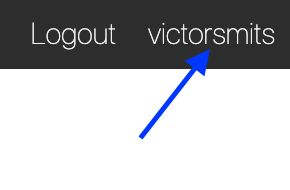
\includegraphics[width=0.4\textwidth,center]{Figures/us7-1}
	\caption{Bouton de navigation vers le profil}
\end{figure}

\vspace{\baselineskip}
\begin{figure}[h]
	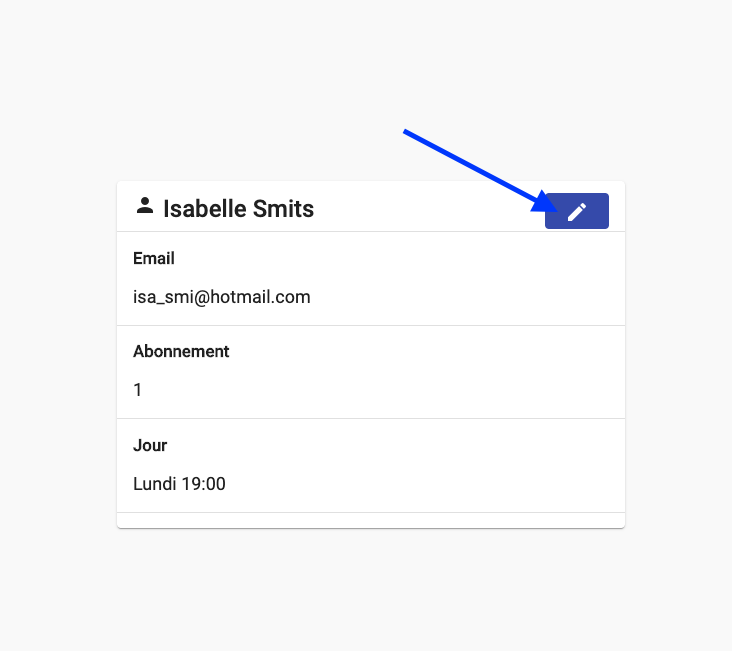
\includegraphics[width=0.4\textwidth,center]{Figures/us8-1}
	\caption{Bouton de modification du profil}
\end{figure}

\newpage
\begin{figure}[h]
	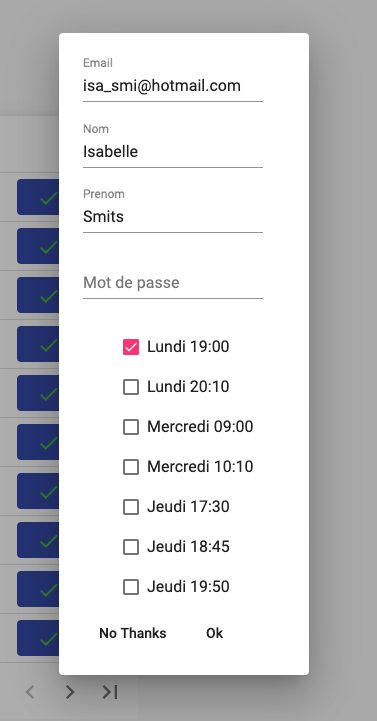
\includegraphics[width=0.4\textwidth,center]{Figures/us8-2}
	\caption{Fenêtre de modification des données du profil}
\end{figure}

\vspace{\baselineskip}
\subsubsection{Script concernés}
	\begin{itemize}
		\item \Href{https://github.com/victorsmits/Aquabike/blob/master/backend/src/Controller/ProfileController.php}{ProfileController.php}
		\item \Href{https://github.com/victorsmits/Aquabike/blob/master/backend/templates/registration/profile.html.twig}{profile.html.twig}
		\item \Href{https://github.com/victorsmits/Aquabike/blob/master/backend/src/Entity/Person.php}{Person.php}
	\end{itemize}